
%(BEGIN_QUESTION)
% Copyright 2011, Tony R. Kuphaldt, released under the Creative Commons Attribution License (v 1.0)
% This means you may do almost anything with this work of mine, so long as you give me proper credit

Suppose the operator of this distillation process calls you to investigate a high-level alarm he is receiving on LAH-58.  He doesn't think this should be happening, because LIC-38 registers a liquid level of 5'-1" in the bottom of the tower, which is a bit less than setpoint (5'-4").  Your first test is to measure the current signal from LT-38a, and you find that to be 10.67 mA (LT-38a is ranged 3'-0" to 8'-0"):

$$\includegraphics[width=15.5cm]{i0001rx01.eps}$$

Identify which faults could account for this problem:

% No blank lines allowed between lines of an \halign structure!
% I use comments (%) instead, so that TeX doesn't choke.

$$\vbox{\offinterlineskip
\halign{\strut
\vrule \quad\hfil # \ \hfil & 
\vrule \quad\hfil # \ \hfil & 
\vrule \quad\hfil # \ \hfil \vrule \cr
\noalign{\hrule}
%
% First row
{\bf Fault} & {\bf Possible} & {\bf Impossible} \cr
%
\noalign{\hrule}
%
% Another row
LSH-58 failed &  &  \cr
%
\noalign{\hrule}
%
% Another row
LAH-58 failed &  &  \cr
%
\noalign{\hrule}
%
% Another row
LSL-57 failed &  &  \cr
%
\noalign{\hrule}
%
% Another row
LAL-57 failed &  &  \cr
%
\noalign{\hrule}
%
% Another row
LT-38a calibration error &  &  \cr
%
\noalign{\hrule}
%
% Another row
LIC-38 (input) calibration error &  &  \cr
%
\noalign{\hrule}
%
% Another row
FIC-37 (input) calibration error &  &  \cr
%
\noalign{\hrule}
} % End of \halign 
}$$ % End of \vbox

\underbar{file i03566}
%(END_QUESTION)





%(BEGIN_ANSWER)

% No blank lines allowed between lines of an \halign structure!
% I use comments (%) instead, so that TeX doesn't choke.

$$\vbox{\offinterlineskip
\halign{\strut
\vrule \quad\hfil # \ \hfil & 
\vrule \quad\hfil # \ \hfil & 
\vrule \quad\hfil # \ \hfil \vrule \cr
\noalign{\hrule}
%
% First row
{\bf Fault} & {\bf Possible} & {\bf Impossible} \cr
%
\noalign{\hrule}
%
% Another row
LSH-58 failed & $\surd$ &  \cr
%
\noalign{\hrule}
%
% Another row
LAH-58 failed & $\surd$ &  \cr
%
\noalign{\hrule}
%
% Another row
LSL-57 failed &  & $\surd$ \cr
%
\noalign{\hrule}
%
% Another row
LAL-57 failed &  & $\surd$ \cr
%
\noalign{\hrule}
%
% Another row
LT-38a calibration error &  & $\surd$ \cr
%
\noalign{\hrule}
%
% Another row
LIC-38 (input) calibration error &  & $\surd$ \cr
%
\noalign{\hrule}
%
% Another row
FIC-37 (input) calibration error &  & $\surd$ \cr
%
\noalign{\hrule}
} % End of \halign 
}$$ % End of \vbox

It is highly unlikely that LT-38a is at fault because the controller (LIC-38) receives the median-selected signal from {\it three} different level transmitters.  In order for the 10.67 mA signal to be incorrect, at least one of the other two level transmitters (LT-38b or LT-38c) would also have to be experiencing the same calibration error!  In other words, this scenario would require coincidental faults, which are highly unlikely.

%(END_ANSWER)





%(BEGIN_NOTES)

\vskip 10pt

This question is a good candidate for a ``Virtual Troubleshooting'' exercise.  Presenting the diagram to students, you first imagine in your own mind a particular fault in the system.  Then, you present one or more symptoms of that fault (something noticeable by an operator or other user of the system).  Students then propose various diagnostic tests to perform on this system to identify the nature and location of the fault, as though they were technicians trying to troubleshoot the problem.  Your job is to tell them what the result(s) would be for each of the proposed diagnostic tests, documenting those results where all the students can see.

During and after the exercise, it is good to ask students follow-up questions such as:

\begin{itemize}
\item{} What does the result of the last diagnostic test tell you about the fault?
\item{} Suppose the results of the last diagnostic test were different.  What then would that result tell you about the fault?
\item{} Is the last diagnostic test the best one we could do?
\item{} What would be the ideal order of tests, to diagnose the problem in as few steps as possible?
\end{itemize}

%INDEX% Basics, control loop troubleshooting (realistic P&ID shown)
%INDEX% Measurement, level: troubleshooting
%INDEX% Process: distillation, generic (realistic P&ID shown)

%(END_NOTES)

